\documentclass[]{beamer}

\usepackage{beamerthemesplit}
\usepackage{latexsym}
\usepackage{verbatim}
\usepackage{listings}

\usetheme{Warsaw}
\useinnertheme{rectangles}

\title{System Architecture}
\author{The BORG Team}
\institute{University of Groningen}
\date{2012}

%TODO: Replace screenshots of code with actual code.

\begin{document}

\begin{frame}
    \titlepage
    \begin{center}
    \tiny{\url{http://www.ai.rug.nl/crl/}} \\
    \tiny{(Relevant courses: ``Practicum Autonome Systemen'' and ``Robotica'')}
    \end{center}
\end{frame}


\section[Outline]{}
\begin{frame}
    \tableofcontents
\end{frame}


\section{Introduction}
\begin{frame}
    \frametitle{Introduction}
    \begin{itemize}
        \item Developed in November 2010
        \item Current repository: around 3000 Commits
        \item Used and developed by the BORG Team
        \item Used for Robtica and PAS courses
    \end{itemize}
\end{frame}


\section{The Architecture}

\subsection{Overview}
\begin{frame}
    \frametitle{Overview}
    Distributed system consisting of;
    \begin{itemize}
        \item Brain
        \item Behaviors
        \item Memory
        \item (Vision) Modules
    \end{itemize}
\end{frame}

\subsection{Examples}

\begin{frame}
    \frametitle{Simple Configuration Example (1)}
    \begin{center}
        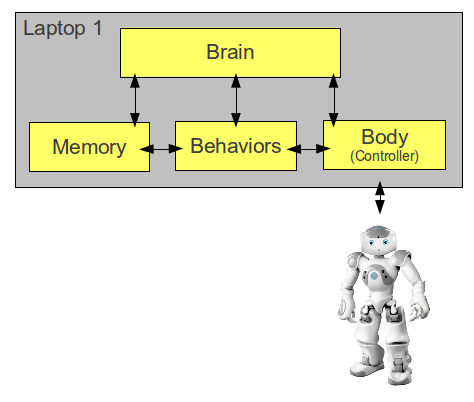
\includegraphics[height=2.2in]{img/arch_example_1.png}
    \end{center}
\end{frame}

\begin{frame}
    \frametitle{Complex Configuration Example (2)}
    \begin{center}
        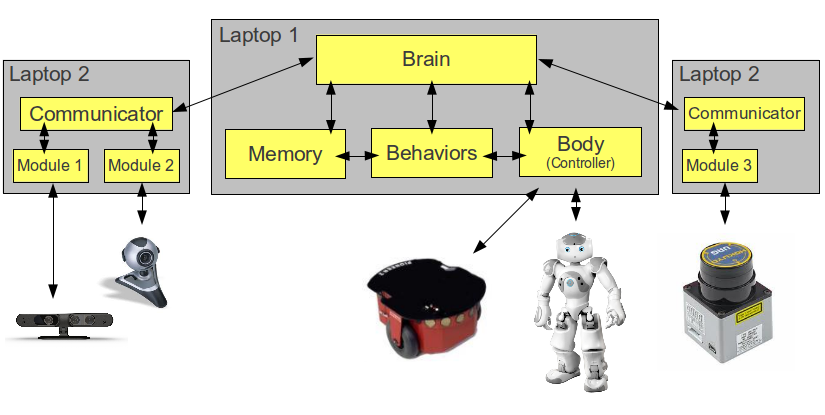
\includegraphics[height=2.2in]{img/arch_example_2.png}
    \end{center}
\end{frame}

\subsection{UML Diagram}
\begin{frame}
    \frametitle{UML Diagram}
    \begin{center}
        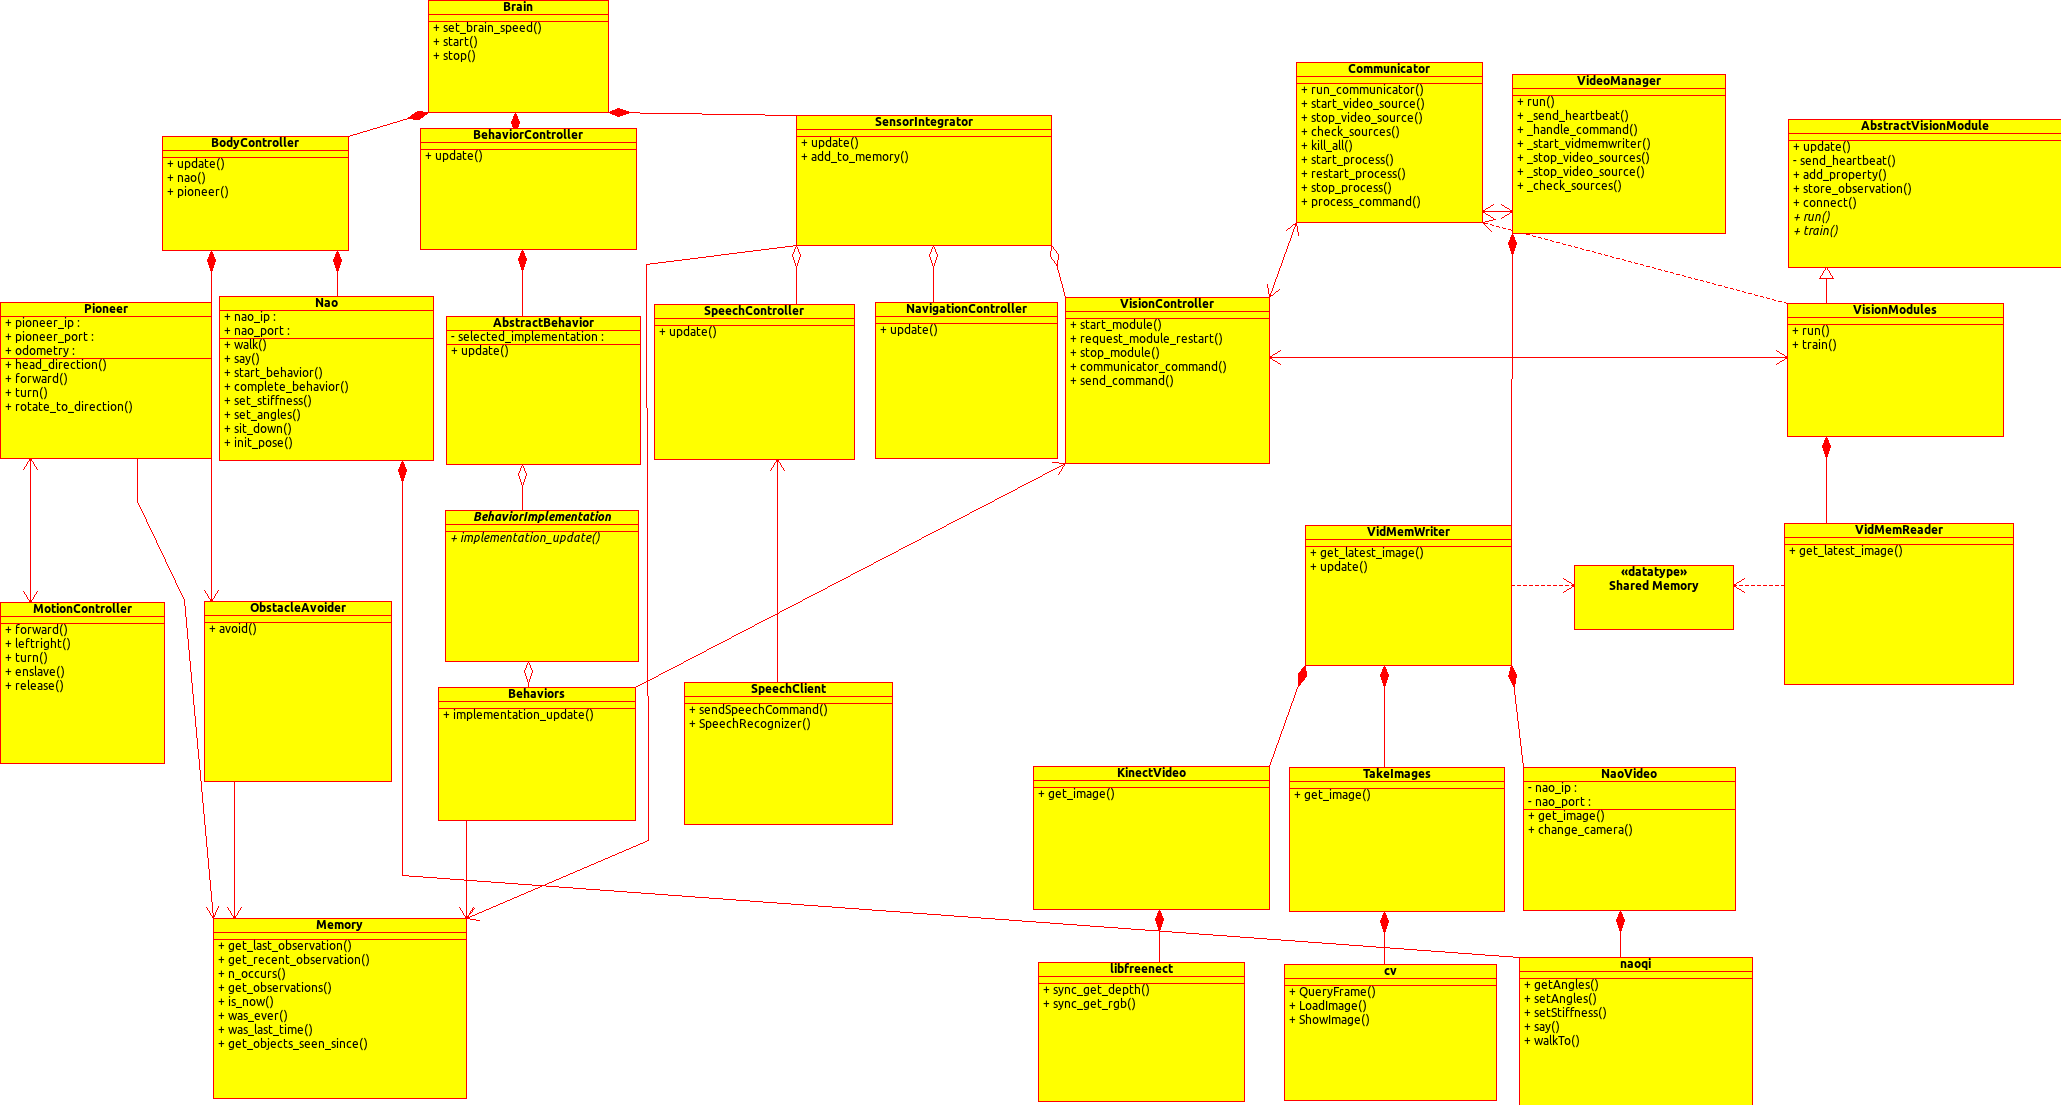
\includegraphics[height=2.2in]{img/architecture.png}
    \end{center}
\end{frame}


\section{Behavior Architecture}

\subsection{Overview}
\begin{frame}
    \frametitle{Behavior Architecture}
    \begin{itemize}
        \item Hierarchical structure
        \item Top behavior, subbehaviors, etc.
        \item Runs on the Brain-laptop
        \item Postconditions, Preconditions, etc.
        \item Base behavior, implementation-specific behaviors.
    \end{itemize}
\end{frame}

\subsection{Hierarchical Structure}
\begin{frame}
    \frametitle{Example (1)}
    \begin{center}
        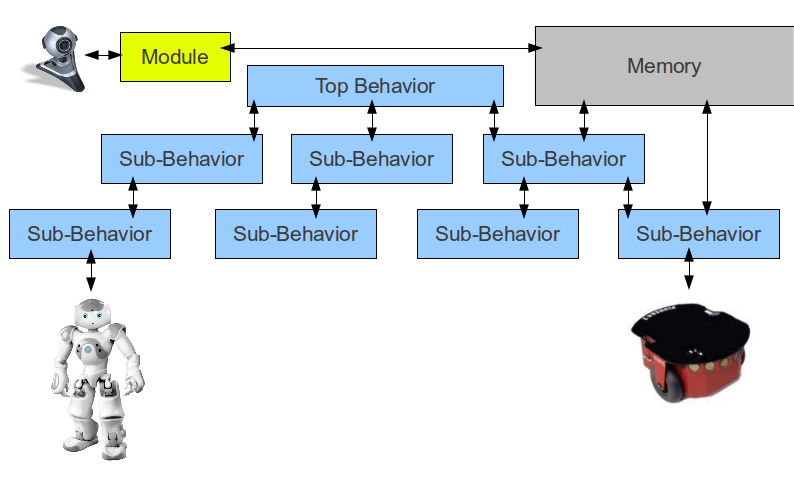
\includegraphics[height=2.2in]{img/behavior_structure_example.png}
    \end{center}
\end{frame}

\subsection{Machine Learning}
\begin{frame}
    \frametitle{Machine Learning}
    \begin{center}
        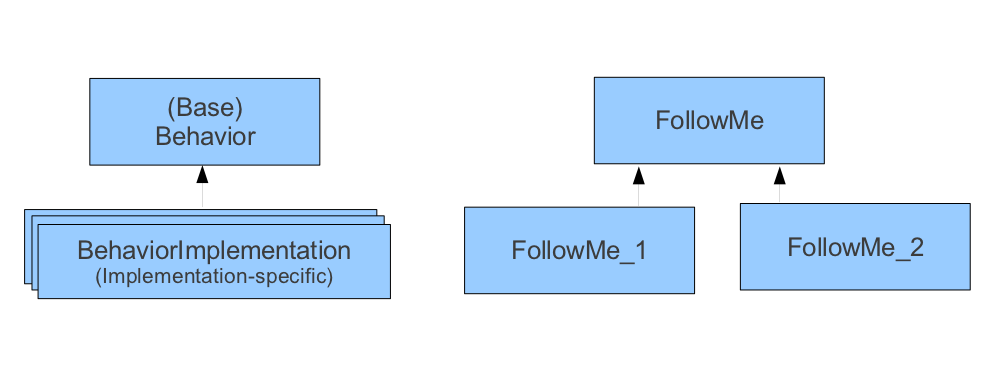
\includegraphics[height=1.5in]{img/behavior_base_implementation.png}
    \end{center}
\end{frame}

\subsection{Conditions}
\begin{frame}
    \frametitle{Conditions}
    \begin{itemize}
        \item Pre-conditions (implementation-specific)
        \item Post-conditions (holds for all implementations)
        \item Exceptions (holds for all implementations)
    \end{itemize}
\end{frame}

\begin{frame}
    \frametitle{Example Conditions}
    Memory lookup, behavior check or a combination of the two:
    \begin{center}
        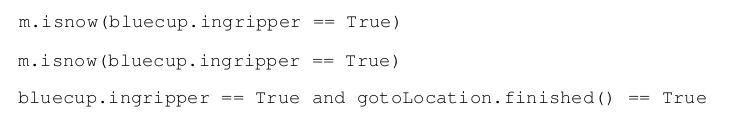
\includegraphics[height=0.7in]{img/conditions.png}
    \end{center}
\end{frame}

\subsection{Implementation Behavior}

\begin{frame}
    \frametitle{Implementation}
    \begin{itemize}
        \item implementation\_update()
        \item implementation\_init(), example:
        \begin{center}
            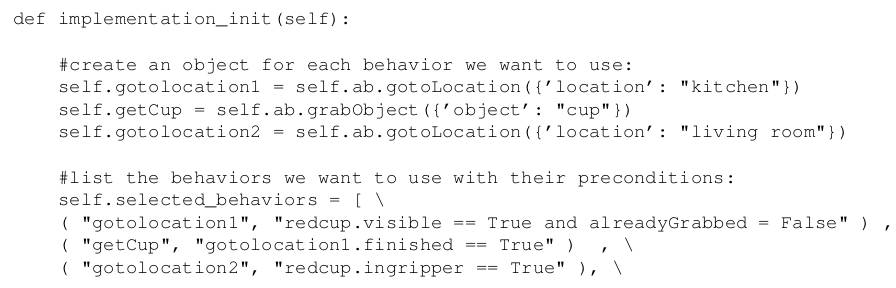
\includegraphics[height=1.5in]{img/implementation_init.png}
        \end{center}
    \end{itemize}
\end{frame}


\subsection{Configuration}
\begin{frame}
    \frametitle{Behaviors Configuration}
    config/behaviors\_config:
    \begin{center}
        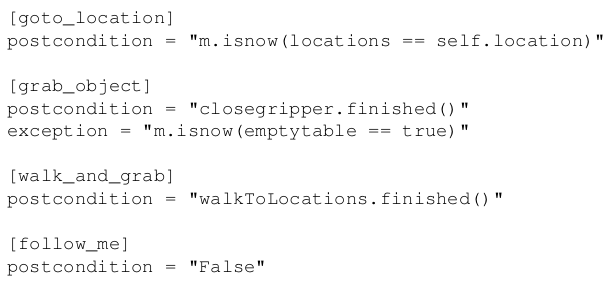
\includegraphics[height=1.5in]{img/behaviors_config.png}
    \end{center}
    Generate behaviors using: \\ \textbf{python src/basebehavior/generate\_behaviors.py}
\end{frame}


\section{Getting Started}

\subsection{Main Configuration File}
\begin{frame}
    \frametitle{Main Configuration File}
    The main configuration file specifies:
    \begin{itemize}
        \item The top behavior (the first behavior to start)
        \item Body configuration (nao, pioneer, etc.)
        \item Speech controller configuration
        \item Vision(/module) controller configuration 
        \item Module and related host settings 
    \end{itemize}
    (Example config files can be found under ``src/config''.)
\end{frame}

\subsection{Installation}
\begin{frame}
    \frametitle{Installation (on the AI machines)}
    \begin{itemize}
        \item Get access to the repository. 
        \item Set enviroment variables.
        \item Clone repository.
    \end{itemize}
\end{frame}

\subsection{Starting the Brain}
\begin{frame}
    \frametitle{Starting the Brain}
    \begin{itemize}
        \item Navigate to the main src directory.
        \item Run the brain using your configuration file: \\
        \textbf{python brain.py ./config/my\_config}
        \item Lookup extra options to use: \\
        \textbf{python brain.py --help}
        \item Using the GUI: \\
        \textbf{./startGUI.sh}
    \end{itemize}
\end{frame}


\subsection{Creating your first behavior}
\begin{frame}
    \frametitle{Creating your first behavior}
    \begin{enumerate}
        \item Edit ``src/config/behaviors\_config'' and add a new behavior (for example ``my\_new\_behavior''). Also, define relevant post-conditions and exceptions.
        \item Generate all behaviors using the \textbf{``python basebehavior/generate\_behaviors.py''} command.
        \item Copy the generated template ``behaviors/my\_new\_behavior/my\_new\_behavior\_x.py'' to  ``behaviors/my\_new\_behavior/my\_new\_behavior\_0.py''.
        \item Edit the new file and add your sub-behaviors (and its preconditions) in the \textbf{implementation\_init()} function.
        \item Add the actual behavior code to the \textbf{implementation\_update()} function.
        \item Create your own config file in the ``src/config'' directory.
    \end{enumerate}
\end{frame}

\begin{frame}
    \frametitle{Creating a more complex behavior}
    \begin{enumerate}
        \item Define the hardware that you require (Nao, Pioneer, etc.)
        \item Define the sensors that you require (e.d. Kinect, Webcam, Laser Range Finder, etc.).
        \item Define the computers and its modules that you are going to use.
        \item Create all behaviors (low-leven, high-level).
        \item Create a new configuration file and add all relevant information.
    \end{enumerate}
\end{frame}



\subsection{Example: Soccer}
\begin{frame}
    \frametitle{Example: Soccer}
    \begin{itemize}
        \item Initial goal; find ball and kick it!
        \item Final goal; play soccer (against other groups)!
        \begin{center}
            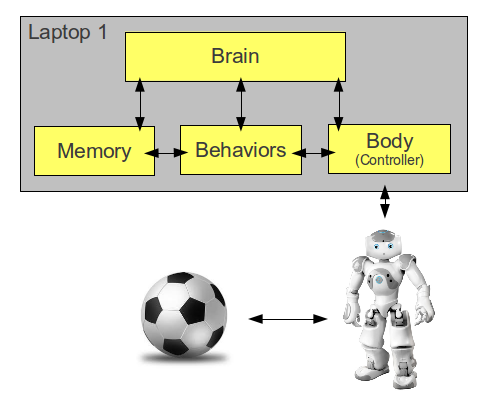
\includegraphics[height=1.5in]{img/arch_soccer.png}
        \end{center}
    \end{itemize}
\end{frame}

\begin{frame}
    \frametitle{Example: Soccer}
    \begin{center}
        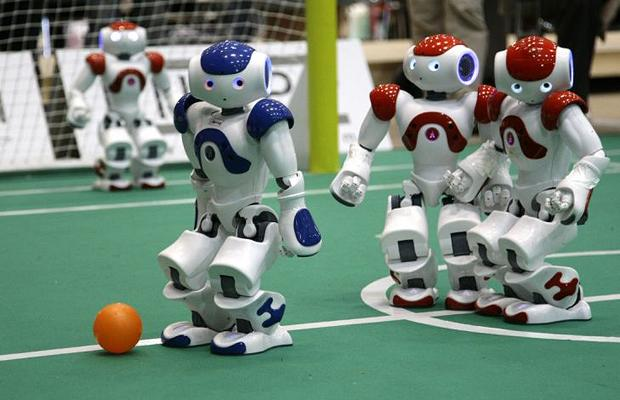
\includegraphics[height=2.0in]{img/soccer.jpg} \\
        \tiny{\url{http://www.telegraph.co.uk}}
    \end{center}
\end{frame}


\section{References}
\begin{frame}
    \frametitle{References}
    \begin{itemize}
        \item \url{http://www.ai.rug.nl/crl}
        \item \url{http://www.ai.rug.nl/robocupathome/}
        \item \url{Repository (Documentation)}
        \item \url{Homerug Mailinglist}
    \end{itemize}
\end{frame}


\end{document}
